\paragraph{QuizziPedia::Front-End::ModelViews::UserDetailsModelView}
		
		\label{QuizziPedia::Front-End::ModelViews::UserDetailsModelView}
		
		\begin{figure}[ht]
			\centering
			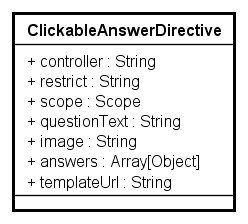
\includegraphics[scale=0.5,keepaspectratio]{UML/Classi/Front-End/QuizziPedia_Front-end_Templates_ClickableAnswerTemplate.png}
			\caption{QuizziPedia::Front-End::ModelViews::UserDetailsModelView}
		\end{figure} \FloatBarrier
		
		\begin{itemize}
			\item \textbf{Descrizione}: classe di tipo modelview la cui istanziazione è contenuta all'interno della variabile di ambiente \$scope di \textit{Angular.js\ped{G}}. All'interno di essa sono presenti le variabili e i metodi necessari per il \textit{Two-Way Data-Binding\ped{G}} tra la view \texttt{UserView} e il controller \texttt{UserDetailsController};
			\item \textbf{Utilizzo}: viene utilizzata per effettuare il \textit{Two-Way Data-Binding\ped{G}} tra la view \texttt{UserView} e il controller \texttt{UserDetailsController} rendendo disponibili variabili e metodi;
			\item \textbf{Relazioni con altre classi}: 
			\begin{itemize}
				\item \textit{IN} \texttt{UserView}: view contenente le direttive dei dati personali dell'utente, delle sue statistiche relative ai questionari e agli allenamenti effettuati e dei questionari a cui è iscritto; 
				\item \textit{IN} \texttt{UserDetailsController}: questa classe permette di ottenere i dati di un utente;
			\end{itemize}
			\item \textbf{Attributi}: 
			\begin{itemize}
				\item \texttt{+ username: String} \\ Attributo che conterrà l'username dell'utente ricercato.
			\end{itemize}
			\item \textbf{Metodi}:
			\begin{itemize}
				\item \texttt{+} \texttt{getUserDetails(username: String): UserDetailsModel} \\ Metodo che permette di ottenere i dati con una chiamata a \texttt{UserDetailsService}; \\
				\textbf{Parametri}:
				\begin{itemize}
					\item \texttt{username: String}: parametro che identifica l'utente del quale saranno scaricati i dati.
				\end{itemize} 
			\end{itemize}
		\end{itemize}
		
			